\subsection{Entry criteria}
\label{sec:entry_criteria}
	In order for the integration process to be performed, a set of preconditions must be met. In particular:
	\begin{description}
		\item[Database] The complete schema provided by the DD must be implemented and tested. The database access system must be at 100\% of its development, and the database must be fully accessible.
		\item[Application logic] Referencing to the components designed in section \textit{2.2 - Component view} of the DD, they must all be unit tested before their integration starts. In addition, their development completion ratio must be so that all the functionalities needed for the integration are already fully developed. 
		% TODO? This approximately translates in the following completion thresholds: <list>
	\end{description}
	Once begun, the integration testing follows and guides the development, as explained in \autoref{sec:integration_testing_strategy}. % FIXME check correctness and add link

\subsection{Elements to be integrated}
	As explained in the DD, the three layers in which the system is divided are characterized as follows.
	\begin{description}
		\item[Data] A database holds and give access to all the data needed by the application. As anticipated in \autoref{sec:entry_criteria}, this layer do not participate actively in the integration process. Indeed, since its development isn't particularly demanding in terms of resources, it is assumed to be already completed once the integration begins. This way, every logic component will be able to access the data layer during the unit testing phase, and integrate with it as a prerequisite for the proper integration phase.
		\item[Application logic] The components on which most of the integration effort will be spent are those intensively described in section \textit{2.2 - Component view} of the DD. These represent the main software components of the system and are responsible to provide the functionalities required by it. In particular, the integration will proceed on two different abstraction layers (one considering only macro-components, the other considering the internal interactions among sub-components), and a particular attention will be paid for the sub-components residing on different machines (e.g.: server and client).
		\item[View] The view layer won't be affected by the integration process. It will be unit tested during its development, and since its interactions takes place only with a single application logic component, it will be straightforward and won't need a delicate testing. The view functioning will be however tested during the more general \textit{system testing} phase. % FIXME ok? Old notes: view unit tested, integration done at the end??, but then why not tested? / main focus on application logic, view just unit tested because dumbly integrated to the rest.
	\end{description}

	As a result, the set of components to be considered for the integration testing become definite:
	\begin{itemize}
		\item \textbf{User Location Handler}
		\item \textbf{User Management server-side} with subcomponents: Profile Manager, License Manager
		\item \textbf{User Management client-side} with subcomponent: User Handler
		\item \textbf{Access Manager}
		\item \textbf{Car Location Handler}
		\item \textbf{Car Manager}
		\item \textbf{Parking Manager}
		\item \textbf{Car Employment Manager}
		\item \textbf{Backend Manager client-side} with subcomponent: Admin Handler
		\item \textbf{Backend Manager server-side} with subcomponent: Backend Manager
		\item \textbf{Operator Location Handler}
		\item \textbf{Maintenance Manager client-side} with subcomponent: Operator Handler
		\item \textbf{Maintenance Manager server-side} with subcomponents: Emergency Report Handler, Report Status Handler, Dispatch Manager
		\item \textbf{Money Saving Option Manager}
		\item \textbf{Payment Manager}
	\end{itemize}
	

\subsection{Integration testing strategy}
\label{sec:integration_testing_strategy}
	The integration of the system will be guided by a bottom-up approach. This strictly comes from an analysis of the dependency structure of the components diagram provided in the DD, here restructured to better highlight the key subsystems and their connections.
	\begin{figure}[h]
		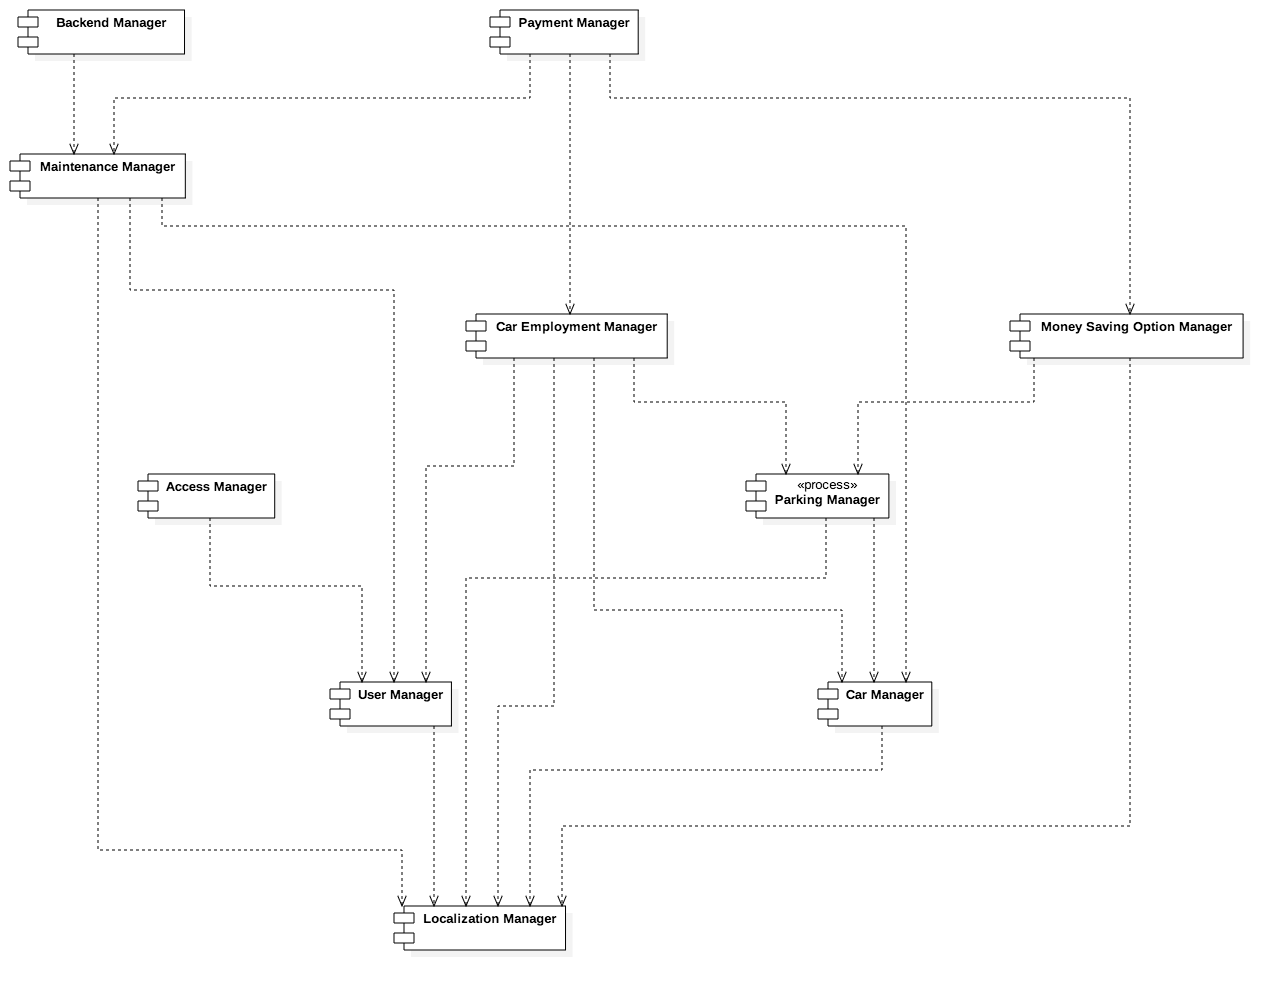
\includegraphics[width=\textwidth, center]{img/integration_strategy/high_level_unravelled.png}
		\caption{Dependency tree of components: high level view.}
	\end{figure}
	\begin{figure}[h]
		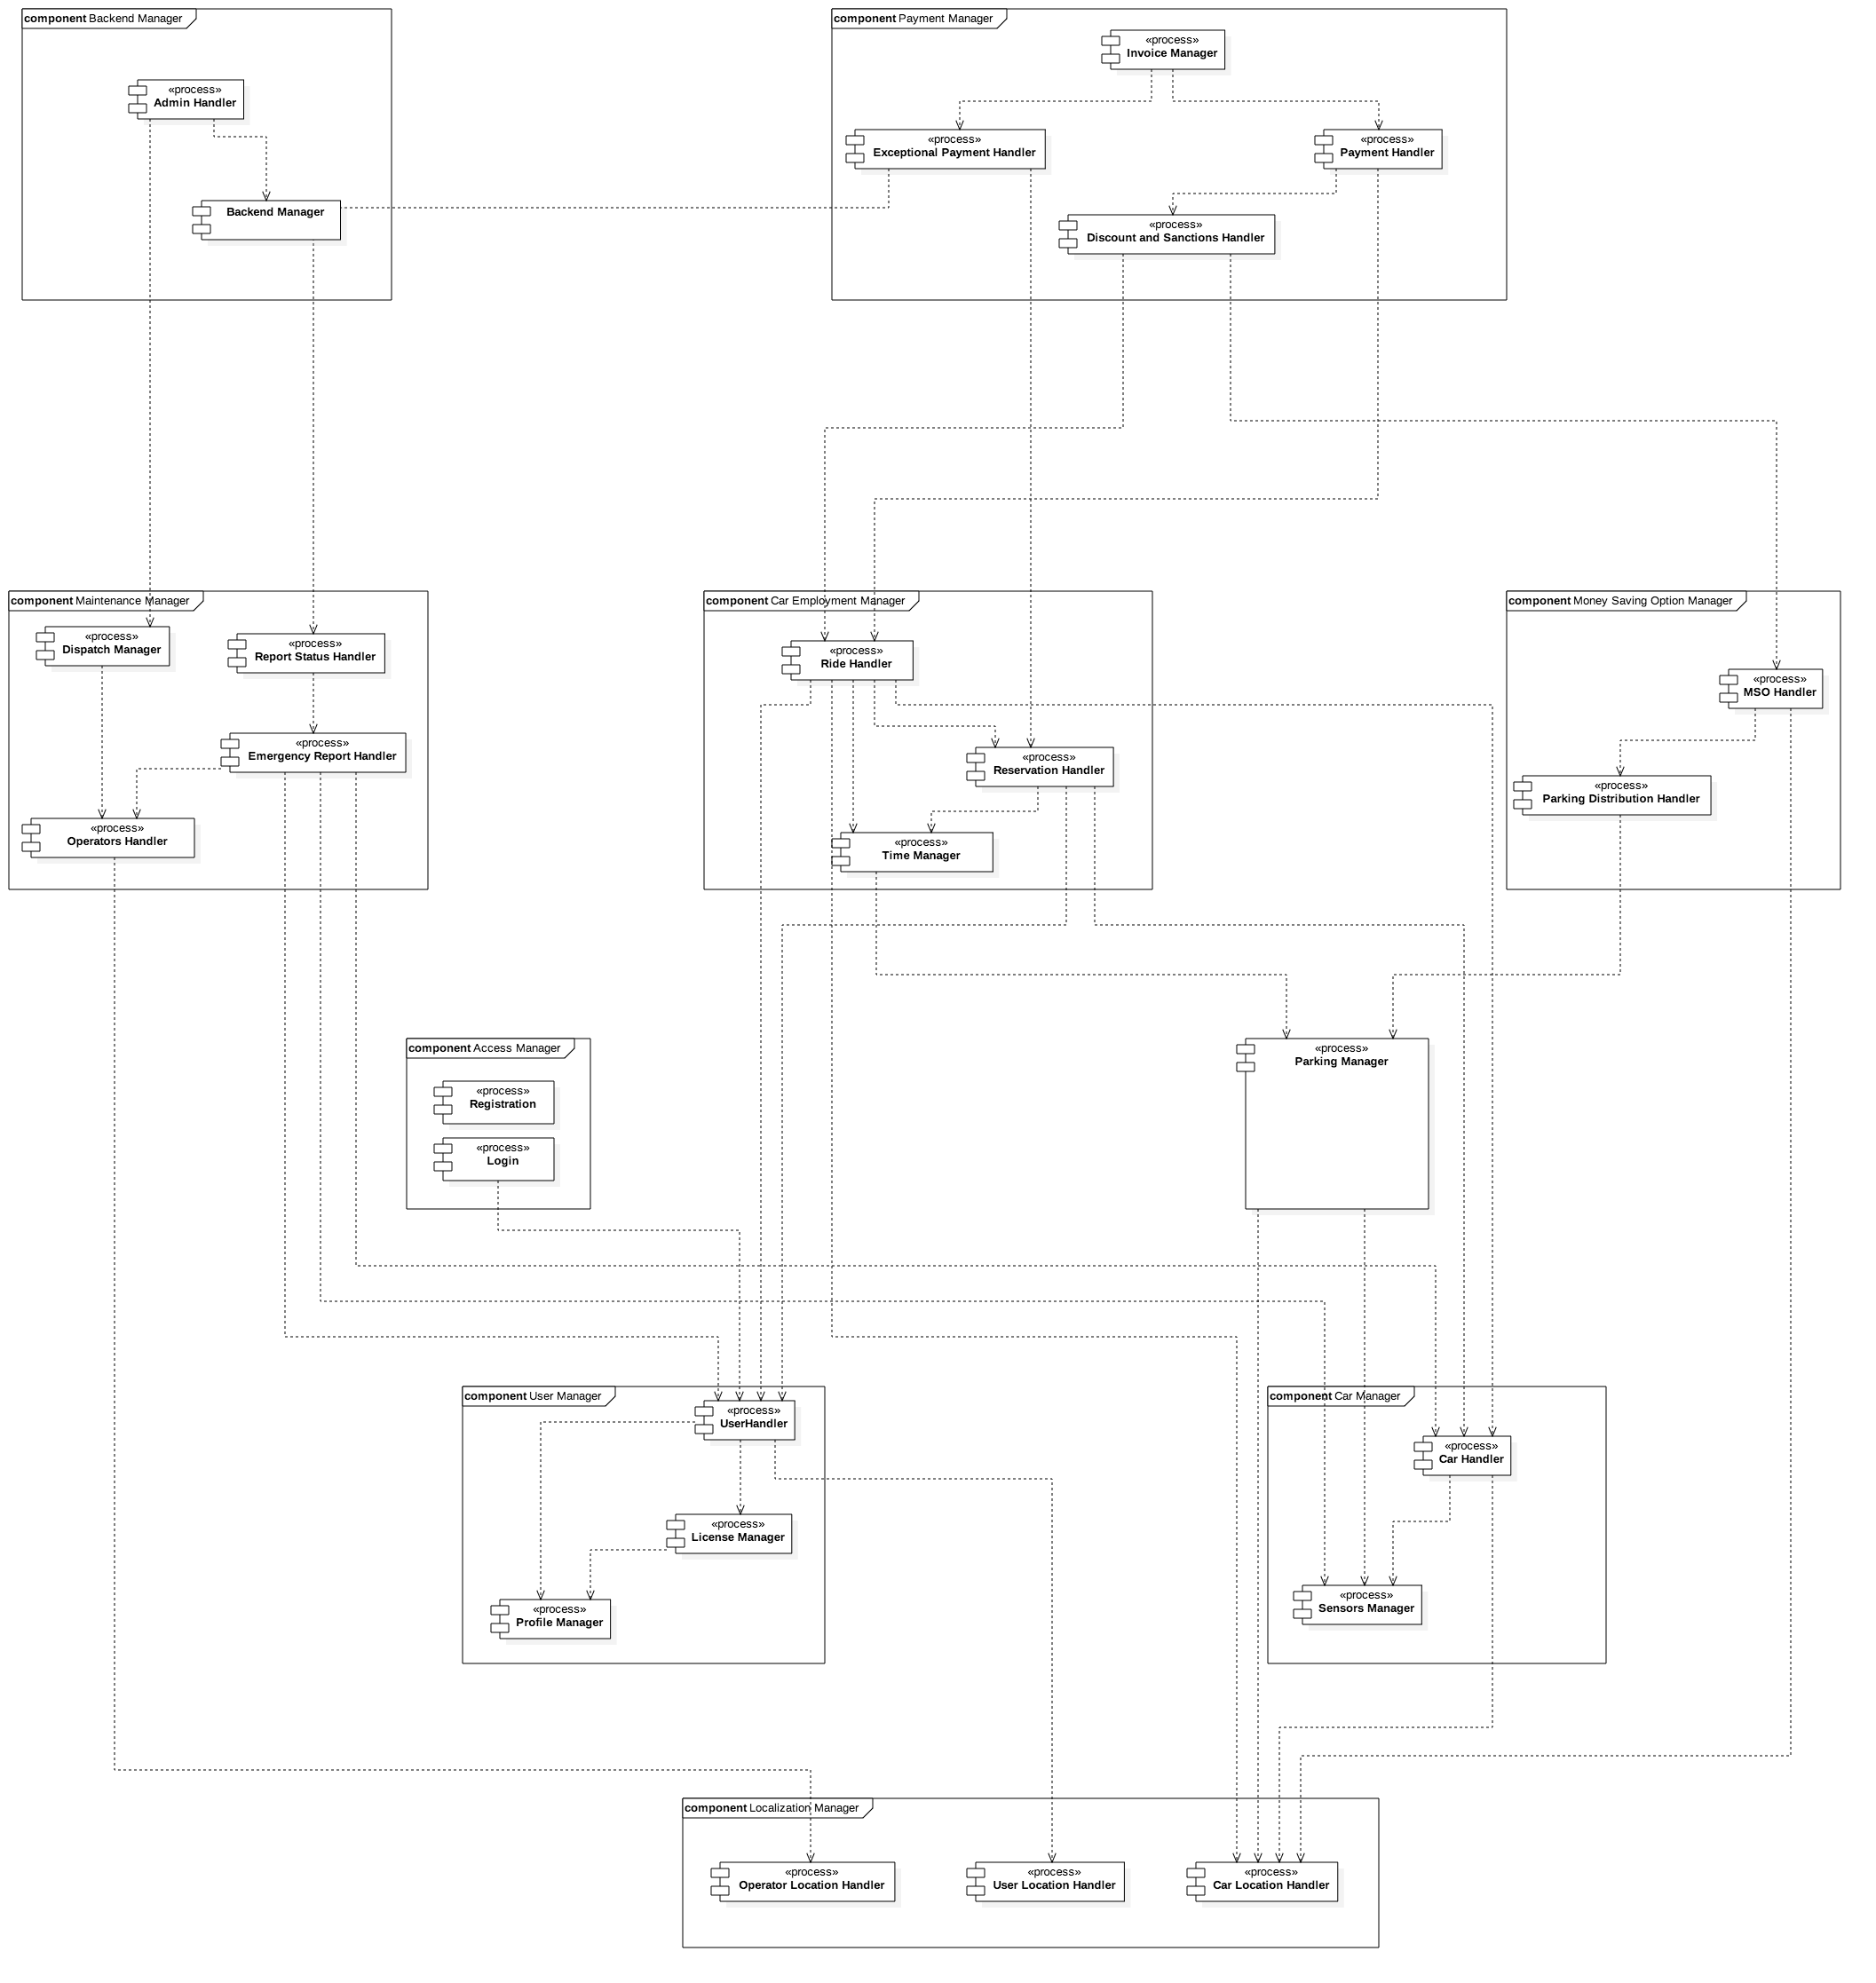
\includegraphics[width=\textwidth, center]{img/integration_strategy/complete_unravelled.png}
		\caption{Dependency tree of components: complete system.}
	\end{figure}
	\FloatBarrier

	This strategy allows for a close interaction between the development phase and the proper testing phase, with a benefit for the quality of the software-to-be as well as for the project management. The goal set with this choice is to make development and testing actually going in parallel during standard operating periods. %% a regime, come si dice!!
	% TODO sth more about it?
	The approach used to integrate the different subcomponents inside a single component is instead selected according to its level of criticality; in particular, the choice revolves around a "nested" bottom-up approach on one hand, and a more complex critical-first approach on the other.
	A criticality analysis underlines the following critical components.
	\begin{itemize}
		\item \textbf{Car Manager.} The integration of the car system software with the underlying hardware and the sensors it is managing involves a moderate number of uncontrollable variables and introduces with them a certain amount of risk. In fact, it is the only point of contact with the actual car, thus becoming the contact point between two rather complex systems.
		\item \textbf{Money Saving Option Manager.} Even if not crucial for the basic functioning of the system, this component is responsible for a large amount of computations, carried on by means of complex algorithms. These must be tested as soon as possible in order to obtain the desired results. In addition, the main algorithm provided by the \textit{Parking Distribution Handler} is designed to be implemented with the not-so-common paradigm of fuzzy logic (see DD \textit{section 3}), and as any not-well-spread development tool, this may suffer for less stability and minor flaws, which must be discovered and managed as soon as possible.
		\item \textbf{Payment Manager.} The payment handling is known to be one of the most critical activities since it involves money transactions. In particular, since the system relies on an external company for the actual payment realizations, its most critical subcomponent is the Invoice Manager, responsible for the interactions with the external \textit{Payment Services Provider}.
	\end{itemize}
	As a result, when the said components are to be developed, their integration will follow a critical-first approach. This increases the chances that any significant problem is found as soon as possible, and therefore should provide benefits in the project management (rescheduling of tasks, reallocation of resources, etc.) aside from the integration process itself.
	% TODO should say here which is the order for these? or in section 2.4?

	The rest of the components, given their less risky nature, will be internally developed following a bottom-up strategy, where the subcomponents are considered all equally-critical and only the "need" dependencies will drive the process.

\subsection{Sequence of component/function integration}
	% see assignment pdf for a non mandatory guide on the structure of this subsection
	% - image of the division bottom up, maybe just with macrocomponents, and explaination
	% - [before or after] details on the single integrations?
	In the present section, the general criteria outlined before are translated to the actual sequence of integration steps to follow in the development and testing of the system. Their presentation will be made exploiting two levels of detail, in a bottom-up fashion: \autoref{sec:software_integration_sequence} refers to the integration of the various sub-components in the context of a particular macro-component, while \autoref{sec:subsystem_integration_sequence} increases the abstraction level, focusing on how the different macro-components will be assembled to form the whole system.

	\subsubsection{Software integration sequence}
	\label{sec:software_integration_sequence}
		% TODO
		% - paragraph for each subsystem (macro component) --> list of images and description (without separations) for the steps, from 2 subcomponents to the whole completed subsystem.
		\paragraphnewline{Localization Manager}
			This component does not require internal integration and will only function as an helper for other components.

		\paragraphnewline{User Manager}
			\begin{itemize}[label={},leftmargin=*,noitemsep,topsep=0pt]
				\item \textit{Internal integration strategy:} bottom-up.
				\item \textit{Integration order:}
					\begin{itemize}[noitemsep]
						\item Profile Manager
						\item License Manager
						\item User Handler
					\end{itemize}
			\end{itemize}
			\begin{figure}[h]
				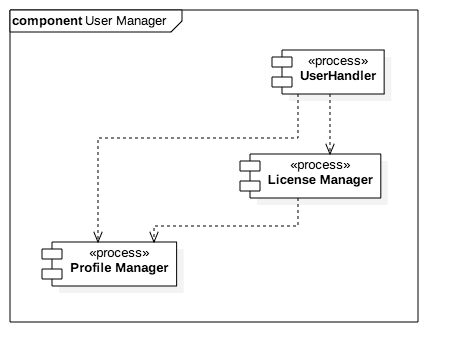
\includegraphics[width=250pt, center]{img/integration_strategy/subcomponents/user_manager.png}
			\end{figure}
		\FloatBarrier

		\paragraphnewline{Car Manager}
			\begin{itemize}[label={},leftmargin=*,noitemsep,topsep=0pt]
				\item \textit{Internal integration strategy:} critical-first.
				\item \textit{Integration order:}
					\begin{itemize}[noitemsep]
						\item Sensors Manager
						\item Car Handler
					\end{itemize}
				\item \textit{Notes: } The integration starts from the Sensors Manager because most of the criticality is related to the communication and management of the system's hardware, functionalities provided by it.
			\end{itemize}
			\begin{figure}[h]
				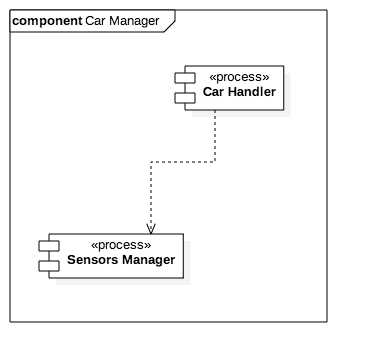
\includegraphics[width=250pt, center]{img/integration_strategy/subcomponents/car_manager.png}
			\end{figure}
		\FloatBarrier

		\paragraphnewline{Parking Manager}
			This component is atomic and thus does not require internal integration.

		\paragraphnewline{Access Manager}
			\begin{itemize}[label={},leftmargin=*,noitemsep,topsep=0pt]
				\item \textit{Internal integration strategy:} bottom-up.
				\item \textit{Integration order:}
					\begin{itemize}[noitemsep]
						\item Login
						\item Registration
					\end{itemize}
				\item \textit{Notes: } The integration starts from the Login because it must be subsequently integrated to the rest of the system, while Registration is independent from it.
			\end{itemize}
			\begin{figure}[h]
				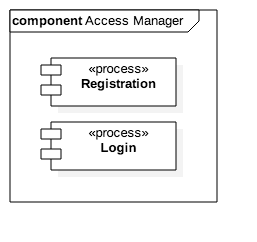
\includegraphics[width=150pt, center]{img/integration_strategy/subcomponents/access_manager.png}
			\end{figure}
		\FloatBarrier

		\paragraphnewline{Car Employment Manager}
			\begin{itemize}[label={},leftmargin=*,noitemsep,topsep=0pt]
				\item \textit{Internal integration strategy:} bottom-up.
				\item \textit{Integration order:}
				\begin{itemize}[noitemsep]
					\item Time Manager
					\item Reservation Handler
					\item Ride Handler
				\end{itemize}
			\end{itemize}
			\begin{figure}[h]
				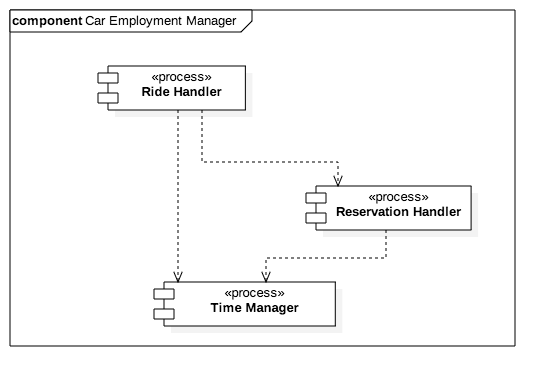
\includegraphics[width=250pt, center]{img/integration_strategy/subcomponents/car_employment_manager.png}
			\end{figure}
		\FloatBarrier

		\paragraphnewline{Money Saving Option}
			\begin{itemize}[label={},leftmargin=*,noitemsep,topsep=0pt]
				\item \textit{Internal integration strategy:} critical-first.
				\item \textit{Integration order:}
					\begin{itemize}[noitemsep]
						\item Parking Distribution Handler
						\item MSO Handler
					\end{itemize}
				\item \textit{Notes: } The Parking Distribution Handler is considered to be the most critical component between the two, since it has to deal with the core MSO algorithm, moreover exploiting not completely supported tools (as FCL for the fuzzy system).
			\end{itemize}
			\begin{figure}[h]
				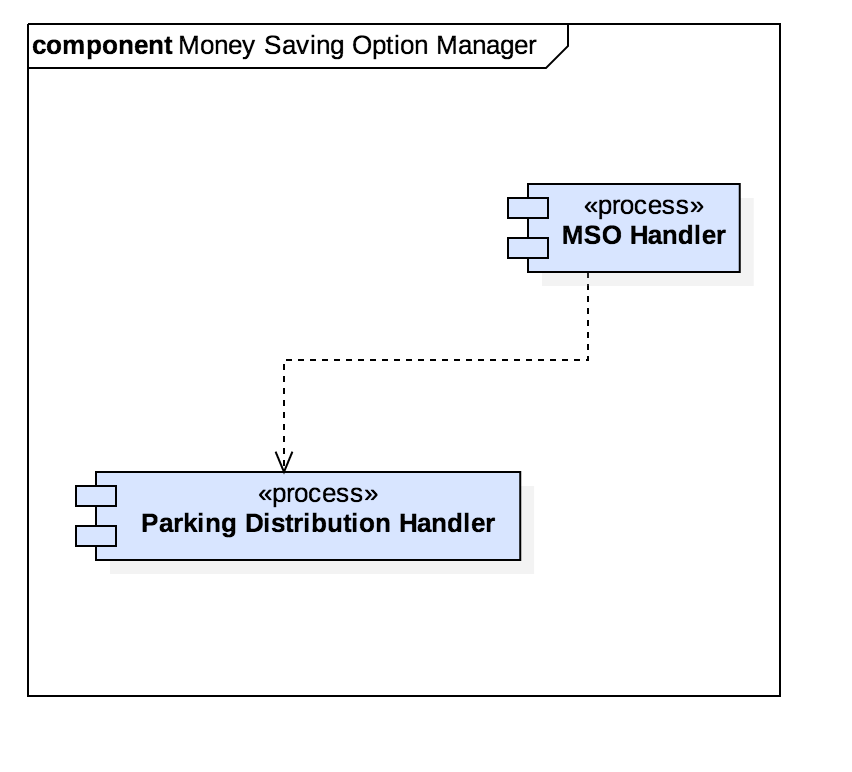
\includegraphics[width=250pt, center]{img/integration_strategy/subcomponents/money_saving_option_manager.png}
			\end{figure}
		\FloatBarrier

		\paragraphnewline{Maintenance Manager}
			\begin{itemize}[label={},leftmargin=*,noitemsep,topsep=0pt]
				\item \textit{Internal integration strategy:} bottom-up.
				\item \textit{Integration order:}
					\begin{itemize}[noitemsep]
						\item Report Status Handler
						\item Emergency Report Handler
						\item Operators Handler
						\item Dispatch Manager
					\end{itemize}
			\end{itemize}
			\begin{figure}[h]
				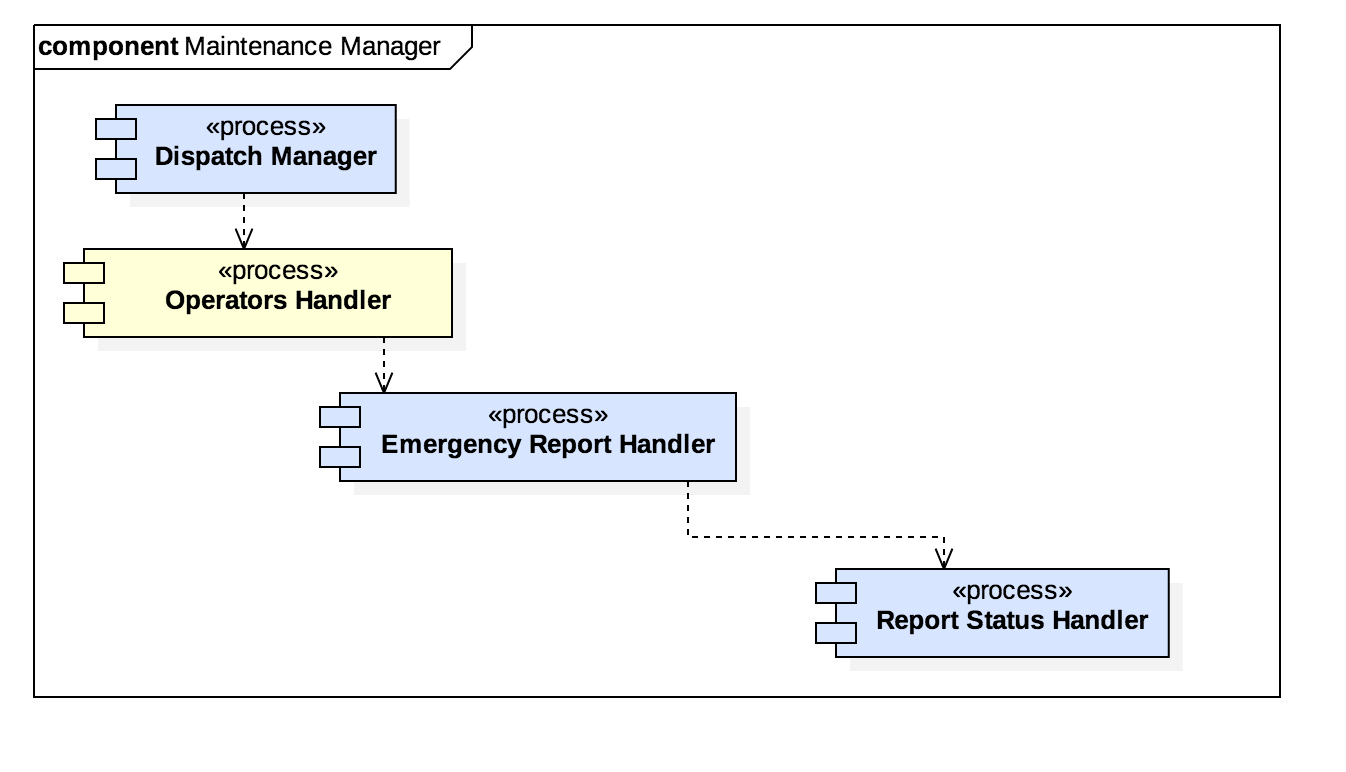
\includegraphics[width=250pt, center]{img/integration_strategy/subcomponents/maintenance_manager.png}
			\end{figure}
		\FloatBarrier

		\paragraphnewline{Payment Manager}
			\begin{itemize}[label={},leftmargin=*,noitemsep,topsep=0pt]
				\item \textit{Internal integration strategy:} critical-first.
				\item \textit{Integration order:}
					\begin{itemize}[noitemsep]
						\item Invoice Manager
						\item Payment Handler
						\item Exceptional Payment Handler
						\item Discount and Sanction Handler
					\end{itemize}
				\item \textit{Notes: } invoice Manager is considered to be the most critical for its responsibility to interact with the external \textit{Payment Services Provider}. The two payment handlers are considered then, and the standard one is privileged because of its importance for the core functioning of the system. Finally the Discount and Sanction Handler is considered to require less effort and is associated to an inferior level of criticality.
			\end{itemize}
			\begin{figure}[h]
				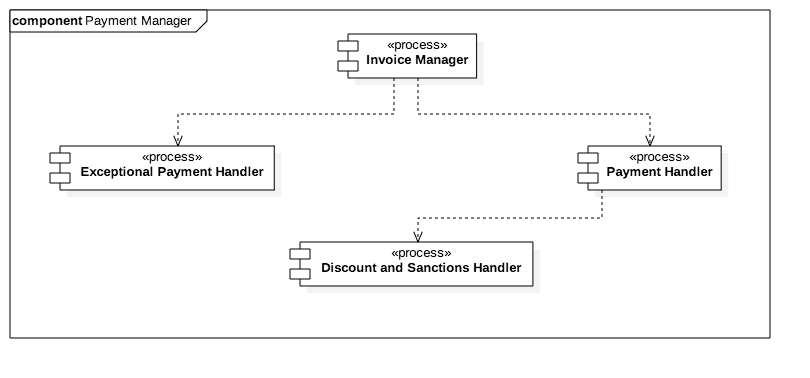
\includegraphics[width=250pt, center]{img/integration_strategy/subcomponents/payment_manager.png}
			\end{figure}
		\FloatBarrier

		\paragraphnewline{Backend Manager}
			\begin{itemize}[label={},leftmargin=*,noitemsep,topsep=0pt]
				\item \textit{Internal integration strategy:} bottom-up.
				\item \textit{Integration order:}
					\begin{itemize}[noitemsep]
						\item Backend Manager
						\item Admin Handler
					\end{itemize}
			\end{itemize}
			\begin{figure}[h]
				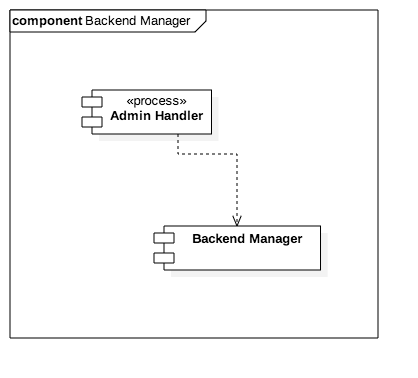
\includegraphics[width=250pt, center]{img/integration_strategy/subcomponents/backend_manager.png}
			\end{figure}
		\FloatBarrier

	\subsubsection{Subsystem  integration  sequence}
	\label{sec:subsystem_integration_sequence}
		% TODO
		% - list of integration steps for each subsystem until the whole system is completed
